
\section*{Problema P11.19}

\renewcommand*\thesection{11.19}
\numberwithin{equation}{section}

\begin{center}
    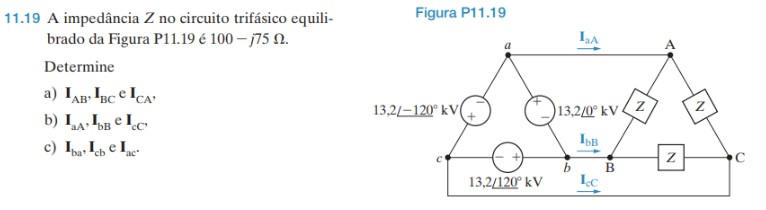
\includegraphics[scale=1.0]{P11.19.jpg}
\end{center}

\subsection*{(a)} 

Observe que a carga $Z_{AB}$ está em paralelo com a fonte de tensão $V_{ab}$. Portanto, a queda de tensão na carga $Z_{AB}$
é $V_{ab}$. Note que o mesmo se aplica para todas as cargas com suas respectivas fontes de tensão. 
\\ Assim,  

\[ I_{AB} = \frac{V_{ab}}{Z_{AB}} = \frac{13200\fase{0}}{100 - j75} = 105.6\fase{36.86} \un{A} \]

\[ I_{BC} = \frac{V_{bc}}{Z_{BC}} = \frac{13200\fase{120}}{100 - j75} = 105.6\fase{156.87} \un{A} \]

\[ I_{CA} = \frac{V_{ca}}{Z_{CA}} = \frac{13200\fase{-120}}{100 - j75} = 105.6\fase{-83.13} \un{A} \]

\subsection*{(b)} 

Aplicando análise nodal no nó (A), temos  

\[ I_{aA} + I_{AB} + I_{CA} = 0 \]

Note que, da maneira que foi definido no item (a), a corrente $I_{CA}$ vai do nó $C$ para o $A$, a corrente
$I_{AB}$ vai do nó $A$ para o $B$. Logo, $I_{CA}$ e $I_{aA}$ entram nó (A), enquanto $I_{AB}$ sai do nó. Corrigindo a equação
nodal, temos  

\[ I_{aA} = I_{AB} - I_{CA} \]

\[ I_{aA} = 105.6\fase{36.86} - 105.6\fase{-83.13} \]

\[ I_{aA} = 84.49 + j63.345 - (12.63 - j104.84) = 71.65 + j168.485 \]

\[ I_{aA} = 183\fase{66.96} \un{A} \]

Aplicamos exatamente o mesmo raciocínio para as demais correntes de fase. \\
Nó (B):

\[ I_{bB} = I_{BC} - I_{AB} \]

\[ I_{bB} = 105.6\fase{156.87} - 105.6\fase{36.86} \]

Extrapolando o resultado de $I_{aA}$,  

\[ I_{bB} = 105.6\sqrt{3}\fase{156.87 + 30} \un{A} \]

\[ I_{bB} = 183\fase{186.87} \un{A} \]

Por último, vamos para o nó (C):

\[ I_{cC} = I_{CA} - I_{BC} \]

\[ I_{cC} = 105.6\fase{-83.13} - 105.6\fase{156.87} \]

\[ I_{cC} = 105.6\sqrt{3}\fase{-83.13 + 30} \un{A} \]

\[ I_{cC} = 183\fase{-53.13} \un{A} \]

\subsection*{(c)} 

Usamos a relação entre corrente de fase e corrente de linha.

\[ I_{ba} = \frac{1}{\sqrt{3}}I_{aA}\fase{66.96 - 30} = 105.1\fase{36.96} \un{A} \]

\[ I_{cb} = \frac{1}{\sqrt{3}}I_{bB}\fase{186.87 - 30} = 105.1\fase{156.87} \un{A} \]

\[ I_{ac} = \frac{1}{\sqrt{3}}I_{cC}\fase{-53.13 - 30} = 105.1\fase{-83.13} \un{A} \]



